% consistency-theory.tex

%%%%%%%%%%%%%%%%%%%%%%%%%%%%%%
\begin{frame}
	motivation: for efficiency; by designing dedicated theory for consistency checking
\end{frame}
%%%%%%%%%%%%%%%%%%%%%%%%%%%%%%

%%%%%%%%%%%%%%%%%%%%%%%%%%%%%%
\begin{frame}{Framework}
	% framework
	% \begin{figure}[H]
	% 	\centering  %图片全局居中
	% 	\subfigure[name1]{
	% 	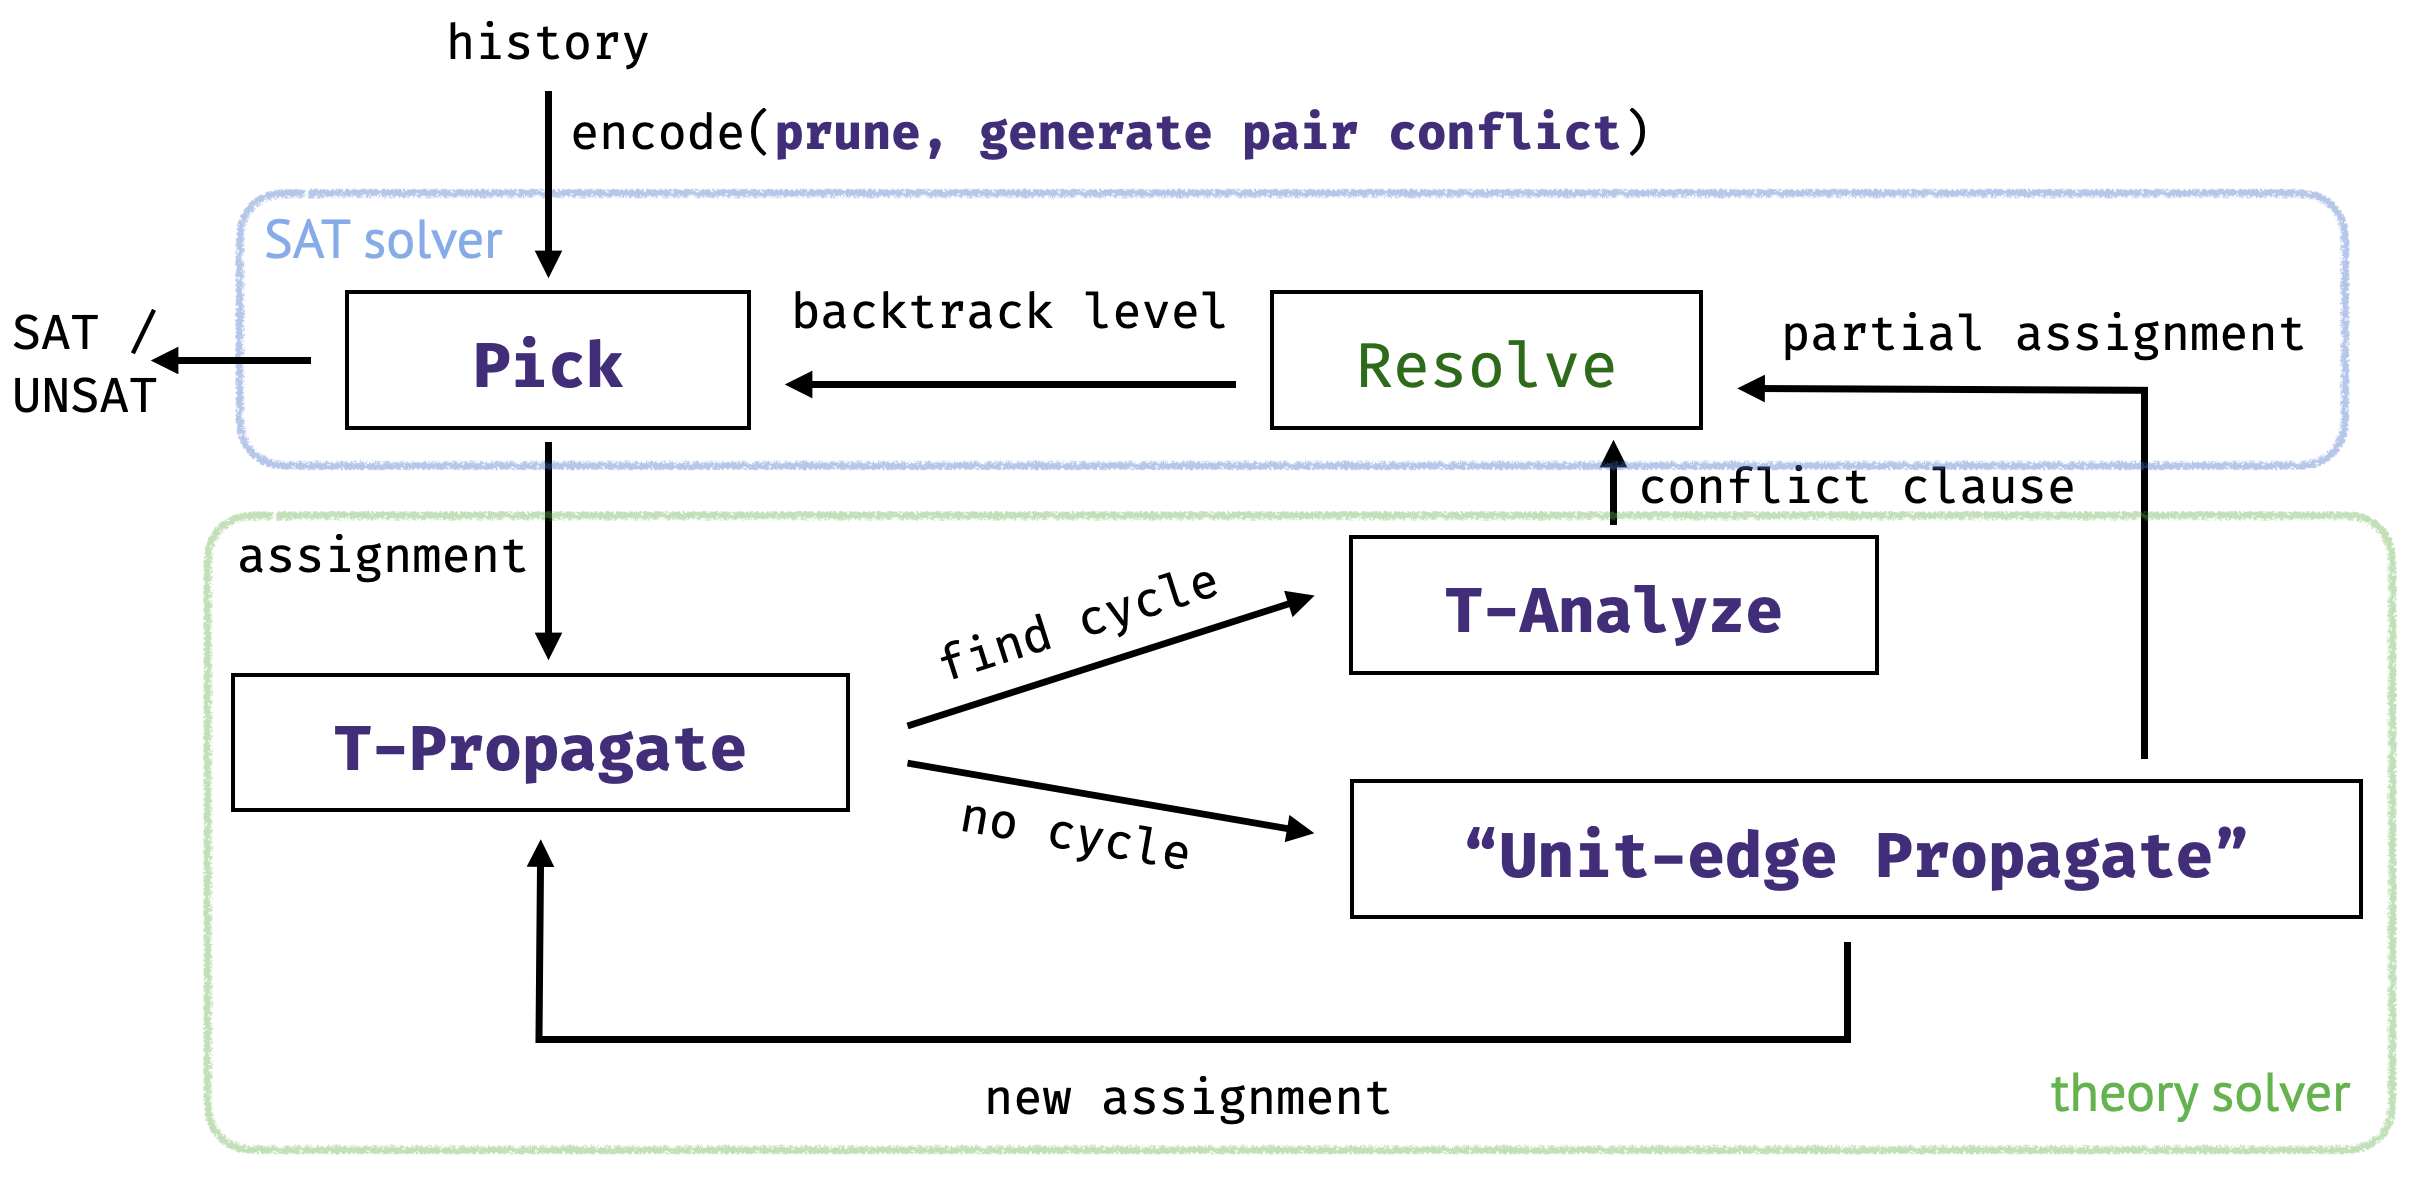
\includegraphics[width=0.45\textwidth]{figs/acyclic-minisat-framework}}
	% 	\subfigure[name2]{
	% 	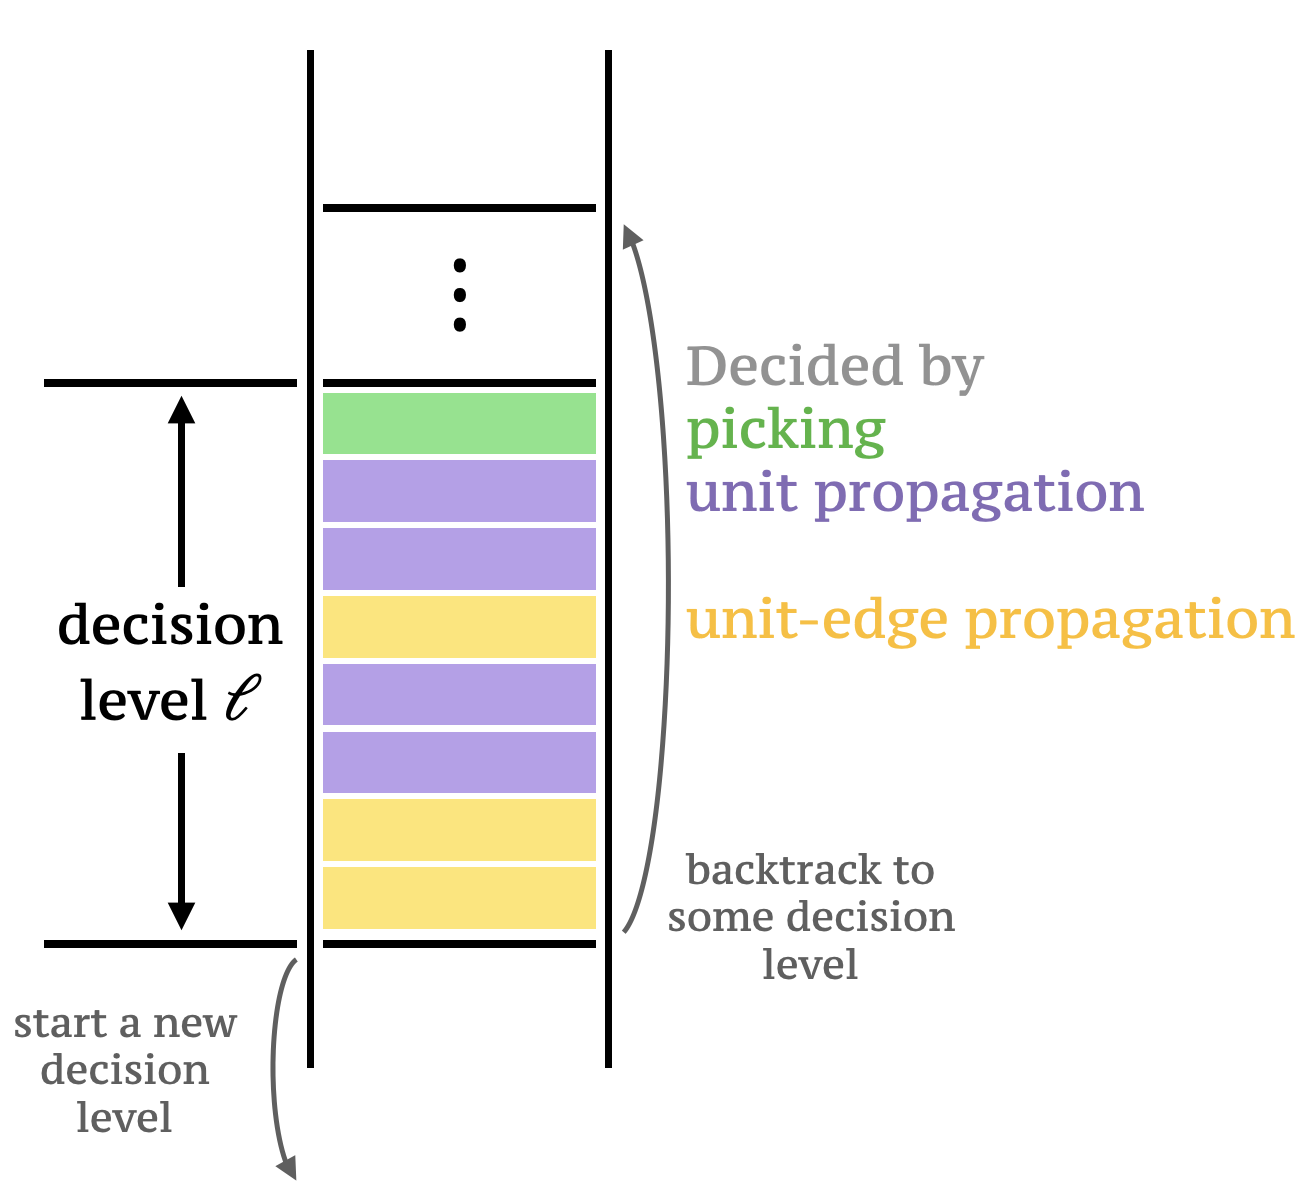
\includegraphics[width=0.45\textwidth]{figs/acyclic-minisat-decision-trail}}
	% \end{figure}

	\begin{figure}[H]
		\centering
		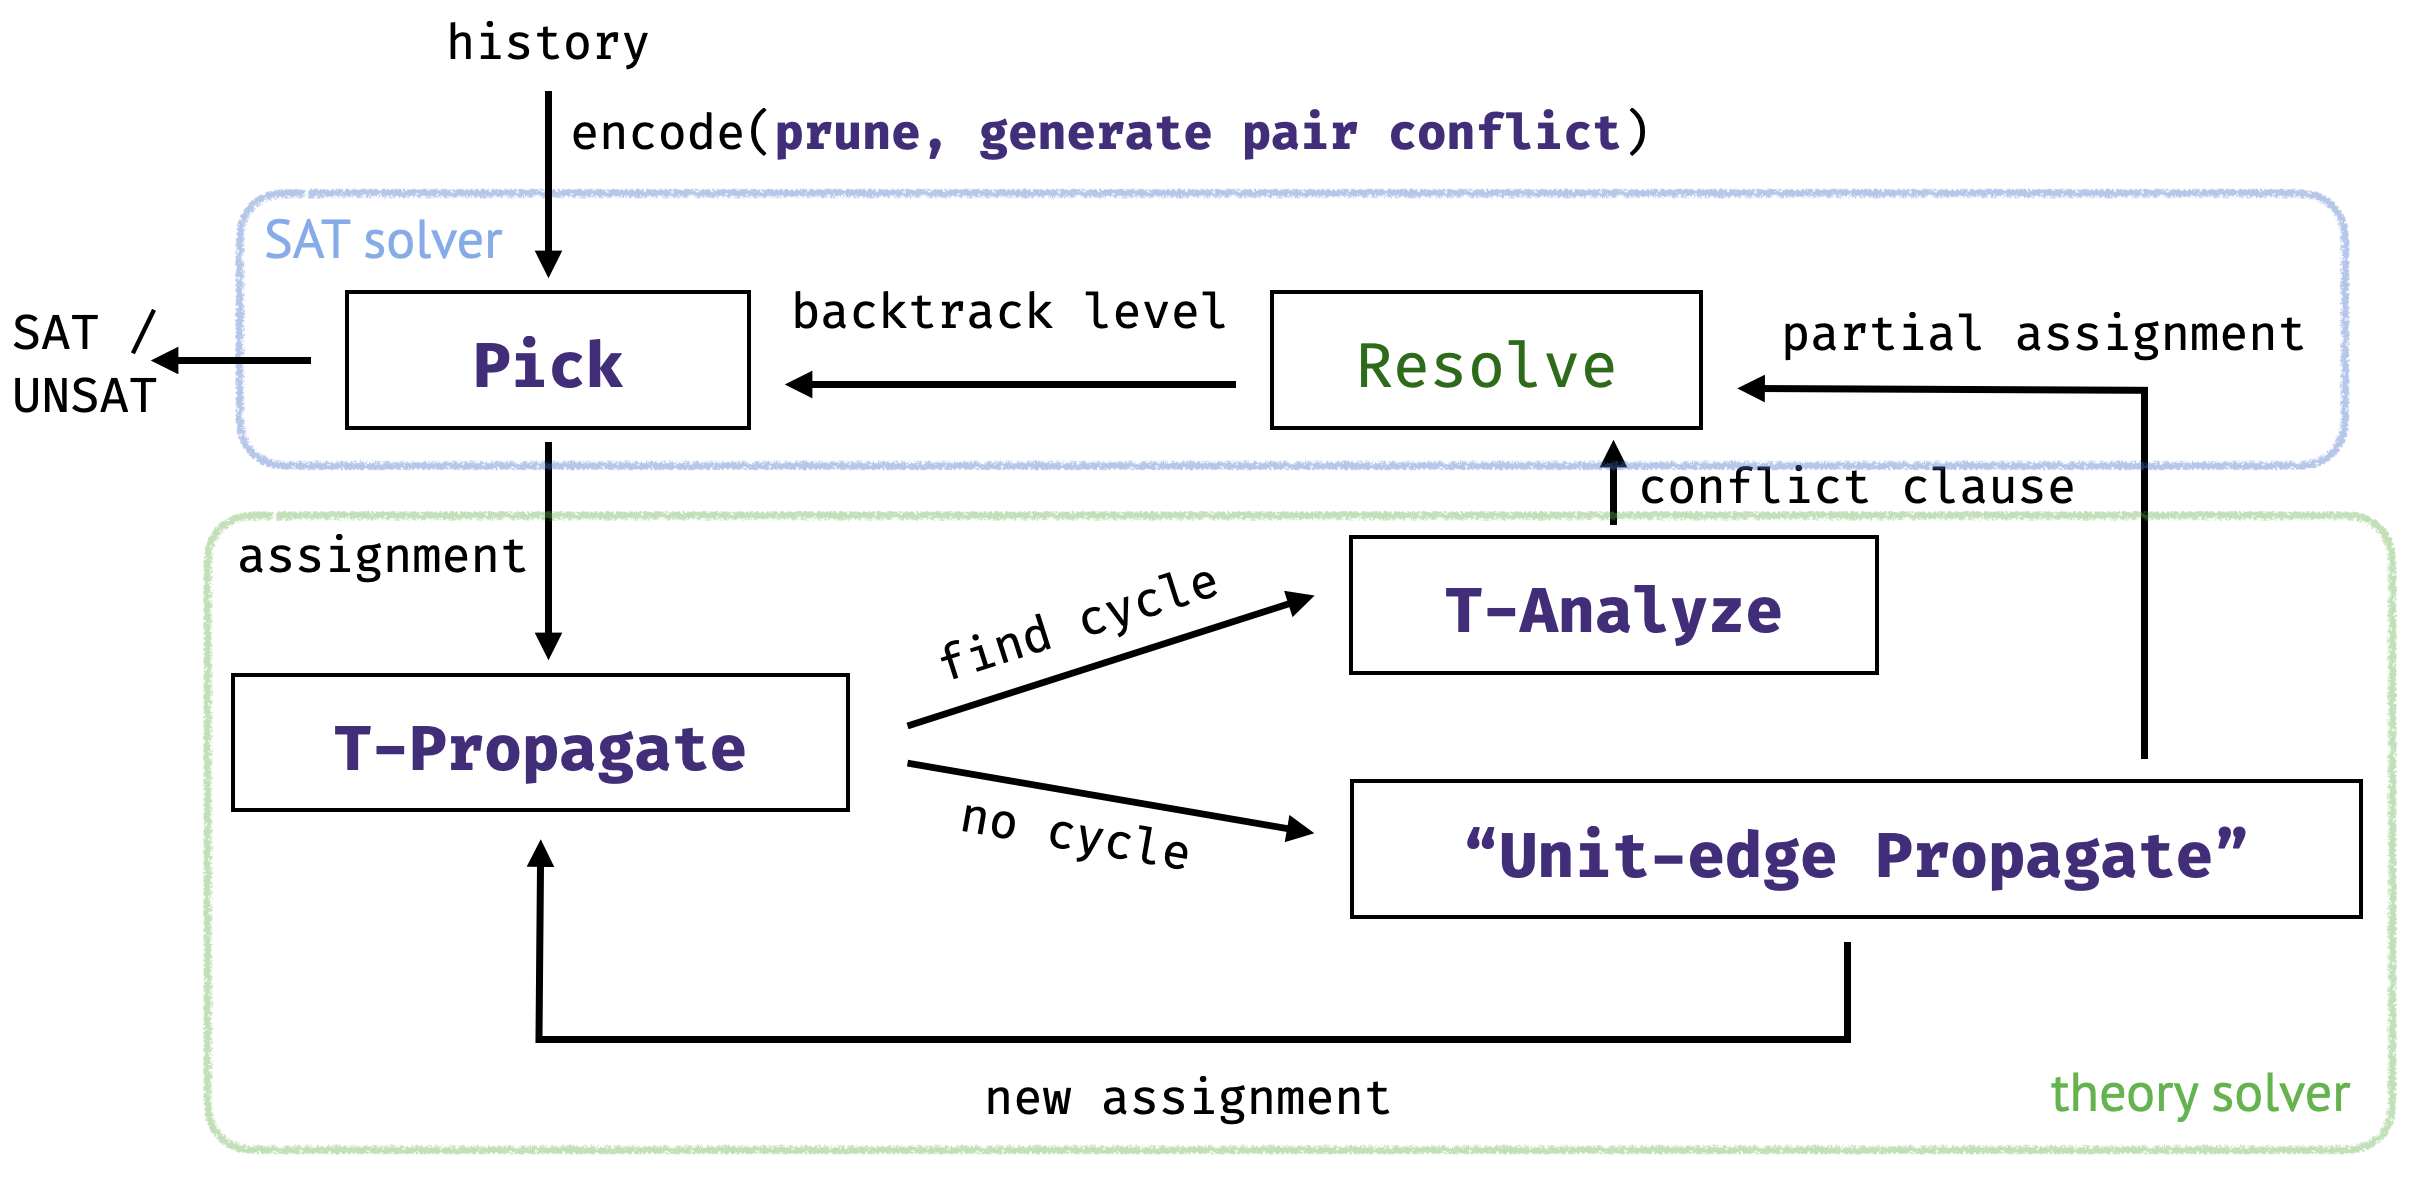
\includegraphics[width=0.6\textwidth]{figs/acyclic-minisat-framework.png}~
		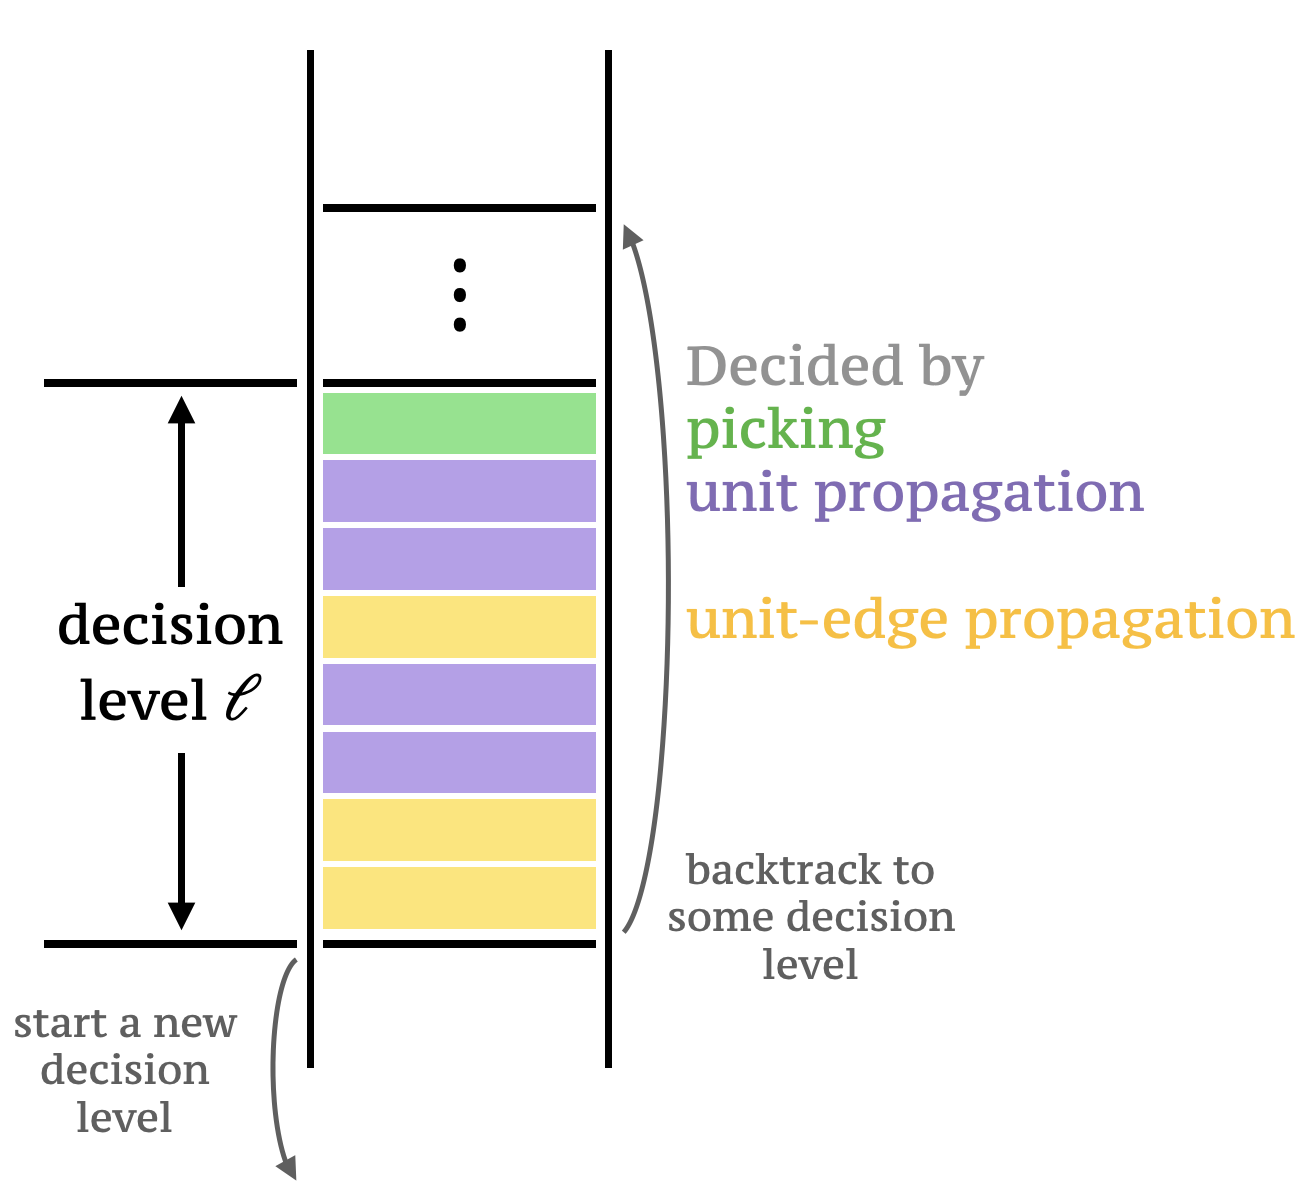
\includegraphics[width=0.36\textwidth]{figs/acyclic-minisat-decision-trail.png}
		\vspace*{0.30cm}
		\footnotesize{framework(left) and decision trail(right)}
	\end{figure}

	% \textcolor[RGB]{71,46,125}{\textbf{#1}}}
	\footnotesize{\textcolor[RGB]{71,46,125}{\textbf{Possible optimizations:}}}
	\scriptsize{
		\begin{itemize}
			\item \textcolor[RGB]{71,46,125}{\textbf{Pick}}: try to assign a variable
			\item \textcolor[RGB]{71,46,125}{\textbf{T}}heory\textcolor[RGB]{71,46,125}{\textbf{-Propagate}}: detect possible cycle upon inserting edges
			\item \textcolor[RGB]{71,46,125}{\textbf{T}}heory\textcolor[RGB]{71,46,125}{\textbf{-Analyze}}: find proper cycle(s)
			\item \textcolor[RGB]{71,46,125}{\textbf{Unit-edge Propagate}}: derive variables from current reachability
		\end{itemize}
	}
\end{frame}
%%%%%%%%%%%%%%%%%%%%%%%%%%%%%%

%%%%%%%%%%%%%%%%%%%%%%%%%%%%%%
\begin{frame}
	1st optimization
\end{frame}
%%%%%%%%%%%%%%%%%%%%%%%%%%%%%%

%%%%%%%%%%%%%%%%%%%%%%%%%%%%%%
\begin{frame}
	2nd optimization
\end{frame}
%%%%%%%%%%%%%%%%%%%%%%%%%%%%%%

%%%%%%%%%%%%%%%%%%%%%%%%%%%%%%
\begin{frame}
	experimental evaluation
\end{frame}
%%%%%%%%%%%%%%%%%%%%%%%%%%%%%%

%%%%%%%%%%%%%%%%%%%%%%%%%%%%%%
\begin{frame}
	what needs to do next
\end{frame}
%%%%%%%%%%%%%%%%%%%%%%%%%%%%%%

%%%%%%%%%%%%%%%%%%%%%%%%%%%%%%
\begin{frame}
	extended to client program verification and robustness verification
\end{frame}
%%%%%%%%%%%%%%%%%%%%%%%%%%%%%%